% !TEX program = tectonic
% Deck « La Chambre, de bout en bout » — la récupération House V1, propre et prouvée.
% Fil : site du Clerk → ZIP → index XML → les 12 FilingType (tableau) → périmètre (cycle de vie)
%      → lisible/scanné par préfixe DocID (prouvé) → paradoxe documents/transactions
%      → cohérence chronologique des portefeuilles (H + P ⊇ T, contrôlée par O/A).
% Tous les chiffres proviennent des tables versionnées 01_v1_house/cache/tables/*.csv et de
% cache/MANIFEST.json — vérifiés par asserts (scratchpad gen_figs_house.py) ; référence en
% commentaire sur chaque slide. Style identique à SLIDES_DONNEES_S1S2.tex.
\documentclass[11pt,aspectratio=169]{beamer}
\definecolor{helec}{HTML}{3B6EA5}   % couleur maîtresse (Chambre électronique)
\usetheme{Madrid}
\usecolortheme[named=helec]{structure}
\setbeamertemplate{navigation symbols}{}
\setbeamertemplate{blocks}[rounded][shadow=false]
\setbeamerfont{frametitle}{series=\bfseries}
\setbeamertemplate{section in toc}[sections numbered]
\setbeamerfont{section in toc}{size=\large}
\usepackage[T1]{fontenc}
\usepackage{lmodern}
\usepackage[utf8]{inputenc}
\usepackage[french]{babel}
\usepackage{booktabs}
\usepackage{xcolor}
\usepackage{graphicx}
\usepackage{fancyvrb}
\usepackage{amssymb}
\usepackage{textcomp}
\usepackage{array}
\usepackage{newunicodechar}
\usepackage{tikz}
\usetikzlibrary{arrows.meta,positioning,calc}
\graphicspath{{figs/}}   % AUTONOME : toutes les images vivent dans 01_v1_house/slides/figs/
\hypersetup{colorlinks=true, urlcolor=helec, linkcolor=white}

% Caractères Unicode → commandes (fontes T1)
\newunicodechar{→}{\ensuremath{\rightarrow}}
\newunicodechar{—}{\textemdash}
\newunicodechar{–}{\textendash}
\newunicodechar{…}{\ldots}
\newunicodechar{·}{\textperiodcentered}
\newunicodechar{≈}{\ensuremath{\approx}}
\newunicodechar{×}{\ensuremath{\times}}
\newunicodechar{≤}{\ensuremath{\leq}}
\newunicodechar{≥}{\ensuremath{\geq}}
\newunicodechar{−}{\ensuremath{-}}
\newunicodechar{✓}{\checkmark}
\newunicodechar{✗}{\ensuremath{\times}}
\newunicodechar{↔}{\ensuremath{\leftrightarrow}}
\newunicodechar{⊇}{\ensuremath{\supseteq}}
\newunicodechar{Σ}{\ensuremath{\Sigma}}
\newunicodechar{∧}{\ensuremath{\wedge}}
\newunicodechar{œ}{\oe}
\newunicodechar{Œ}{\OE}
\newunicodechar{°}{\textdegree}
\newunicodechar{§}{\S}
\newunicodechar{«}{\og}
\newunicodechar{»}{\fg{}}

% Code couleur (repris du deck S1S2 et des figures matplotlib)
\definecolor{helec}{HTML}{3B6EA5}   % Chambre électronique
\definecolor{hocr}{HTML}{A9C5E2}    % Chambre OCR
\definecolor{selec}{HTML}{8E44AD}   % Sénat électronique
\definecolor{socr}{HTML}{CFAEDE}    % Sénat OCR
\definecolor{okgreen}{HTML}{2E8B57}
\definecolor{alertred}{HTML}{C0392B}
\definecolor{warnorange}{HTML}{E67E22}
\definecolor{dataC}{RGB}{176,110,14}  % famille patrimoine (ocre)
\definecolor{grisC}{RGB}{90,90,90}    % cartes neutres (mixable en !10)

% Styles TikZ
\newcommand{\co}[1]{\texttt{#1}}
\tikzset{
  step/.style={rectangle, rounded corners=2pt, draw=#1, line width=0.8pt, fill=#1!8,
               align=center, font=\scriptsize, minimum height=0.72cm},
  bande/.style={rectangle, rounded corners=2pt, draw=#1, line width=0.8pt, fill=#1!8,
                align=center, font=\scriptsize, minimum height=0.62cm},
  arr/.style={-{Latex[length=2mm]}, line width=0.8pt, draw=gray!65},
}

% Tuile chiffre-clé : \tuile{couleur}{gros chiffre}{légende}
\newcommand{\tuile}[3]{%
  \begin{minipage}[t]{0.23\textwidth}\centering
    \colorbox{#1}{\parbox[c][21mm][c]{\dimexpr\linewidth-8pt}{\centering
      {\color{white}\Large\textbf{#2}}\\[0.6mm]
      {\color{white}\footnotesize #3}}}
  \end{minipage}}

% Badge coloré une ligne
\newcommand{\badge}[2]{\colorbox{#1}{\textcolor{white}{\footnotesize\textbf{#2}}}}
\newcommand{\badgel}[2]{\colorbox{#1}{\textcolor{black!80}{\footnotesize\textbf{#2}}}}

\title[La Chambre, de bout en bout]{La Chambre, de bout en bout}
\subtitle{Du site du Clerk au portefeuille de chaque élu — la récupération V1, propre et prouvée}
\author[A.~Lemaire]{Alice Lemaire}
\institute[Ramify]{Document de recherche — livrable Ramify}
\date{Juillet 2026}

\begin{document}

% ── S1 · Titre ──
{\setbeamertemplate{footline}{}
\begin{frame}[plain]
  \titlepage
  \centering
  {\footnotesize reconstruire le portefeuille de chaque membre —
   et le vérifier quand la structure le permet}
\end{frame}}

% ── S2 · Le plan en 10 étapes ── (source : plan canonique validé)
\begin{frame}{Le plan — dix étapes, dans l'ordre du réel}
  \centering
  {\footnotesize\setlength{\tabcolsep}{5pt}\renewcommand{\arraystretch}{1.1}
  \begin{tabular}{l l}
    \textbf{1 · Récupérer} & les 13 index annuels → 35\,377 dépôts recensés \\
    \textbf{2 · Router} & lisible ou scanné — le 1er chiffre du DocID le dit \\
    \textbf{3 · Identifier} & du nom imprimé à l'identifiant stable de l'élu \\
    \textbf{4 · Le cycle de vie} & qui entre, qui sort, qui reste \\
    \textbf{5 · Extraire} & le patrimoine (Schedule A) et les transactions (B) \\
    \textbf{6 · Le portefeuille d'entrée} & la photo de départ de chaque membre \\
    \textbf{7 · Les flux, dédupliqués} & les transactions de toutes les sources \\
    \textbf{8 · Vérifier} & entrée + achats doivent expliquer la sortie \\
    \textbf{9 · Reconstruire} & la série datée du patrimoine, membre par membre \\
    \textbf{10 · Rien d'oublié} & chaque dépôt a un traitement, la somme boucle \\
  \end{tabular}}\\[3mm]
  \colorbox{helec}{\parbox{0.92\textwidth}{\footnotesize\color{white}\centering
    \textbf{deux compteurs, jamais confondus} : on RECONSTRUIT le portefeuille de
    825 membres · on ne peut le VÉRIFIER de bout en bout que pour
    56 d'entre eux — et on sait exactement pourquoi}}
\end{frame}

\section{Étape 1 · Récupérer — les 13 index annuels}
% ── S3 · La source ──
\begin{frame}{La source — le site officiel de la Chambre, une archive par année}
  \begin{columns}[T]
    \begin{column}{0.55\textwidth}\centering
      \fcolorbox{black!25}{white}{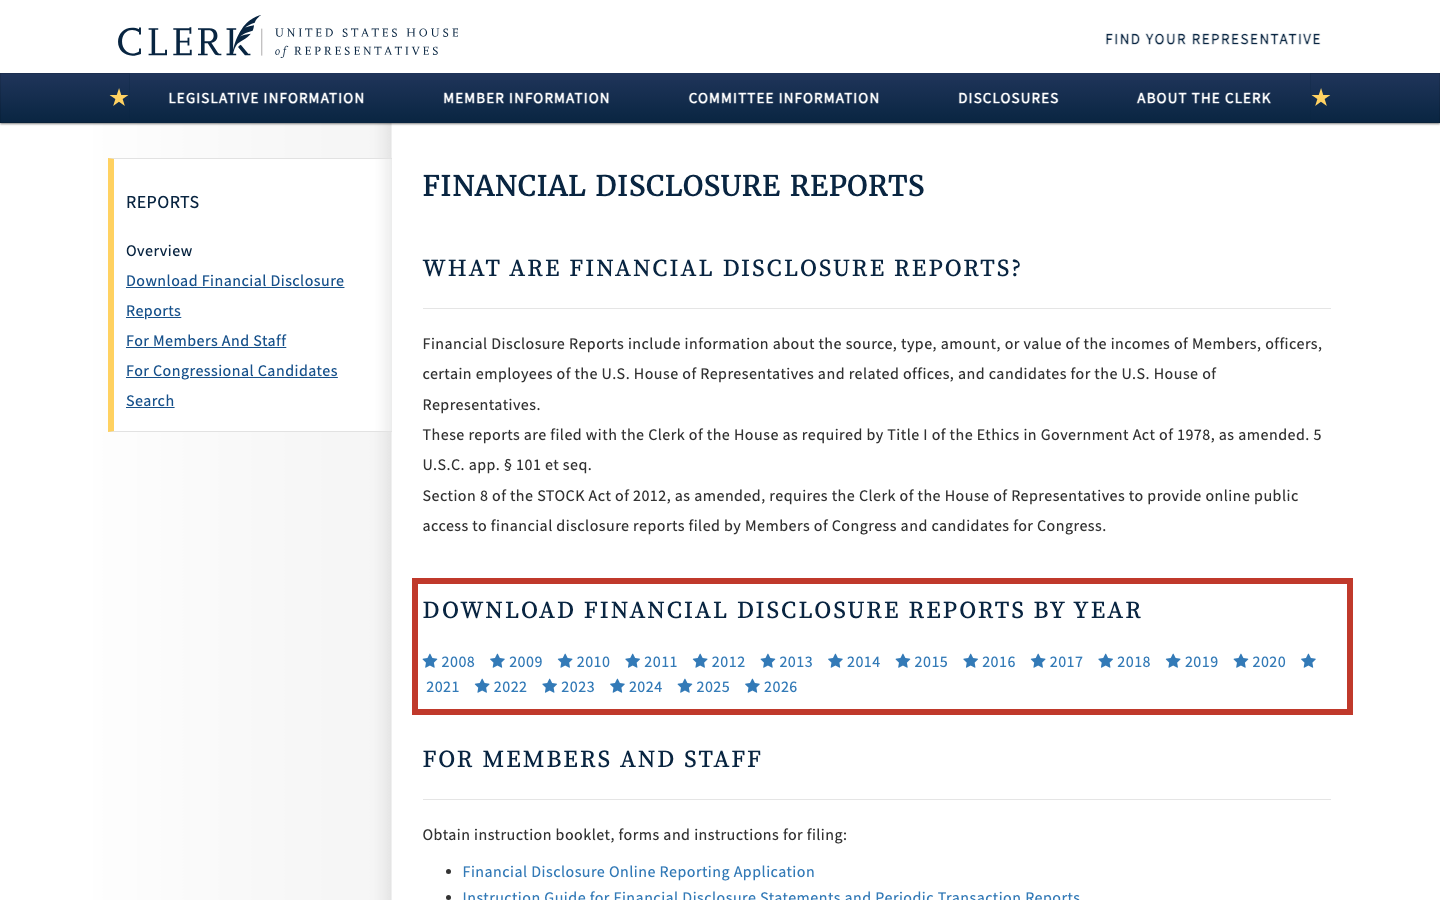
\includegraphics[width=0.95\linewidth]{slides/site_house_clerk.png}}\\[0.8mm]
      {\scriptsize le site du Clerk : un ZIP par année, 2014 → 2026}
    \end{column}
    \begin{column}{0.43\textwidth}\centering
      \fcolorbox{black!25}{white}{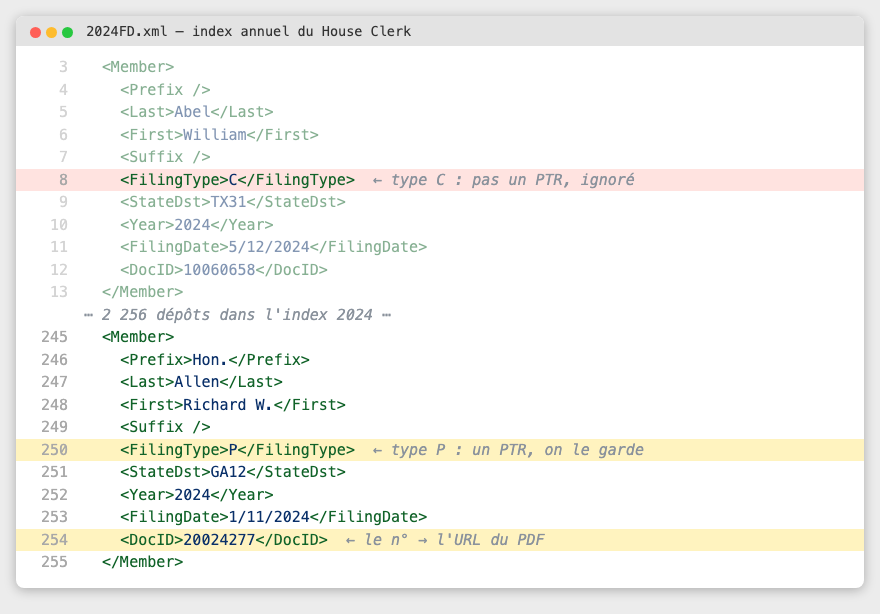
\includegraphics[width=0.95\linewidth]{slides/fichier_index_xml.png}}\\[0.8mm]
      {\scriptsize dans le ZIP : l'index XML — un bloc par dépôt,
       9 champs (nom, type, date, identifiant du document…)}
    \end{column}
  \end{columns}
  \vspace{2.5mm}
  {\footnotesize c'est la \textbf{liste officielle} de tout ce qui a été déposé —
   notre point de départ, et la seule autorité sur « qu'est-ce qui existe »}
\end{frame}

% ── S4 · Le recensement + cas 2014 ── (table 01)
\begin{frame}{35\,377 dépôts recensés — et une année que le site a effacée}
  \centering
  \tuile{helec}{35\,377}{dépôts recensés\\2014 → 2026}\hfill
  \tuile{alertred}{11}{dépôts de 2014\\encore sur le site}\hfill
  \tuile{okgreen}{2\,784}{dépôts de 2014\\dans NOTRE archive}\\[4mm]
  {\footnotesize le site détruit les vieux index (la loi l'y autorise au bout de
   6 ans) : l'année 2014 a presque disparu — elle ne survit que dans la copie
   que nous avons archivée et versionnée. Le recensement final = l'union des deux.}\\[2mm]
  {\scriptsize\color{black!60} seule 2014 est touchée à ce jour ; 2015 → 2026
   sont identiques entre le site et notre archive}
\end{frame}

\section{Étape 2 · Router — lisible ou scanné}
% ── S5 · Le 1er chiffre du DocID ──
\begin{frame}{Deux natures de document — et le 1er chiffre de l'identifiant le dit}
  \begin{columns}[T]
    \begin{column}{0.48\textwidth}\centering
      \fcolorbox{black!25}{white}{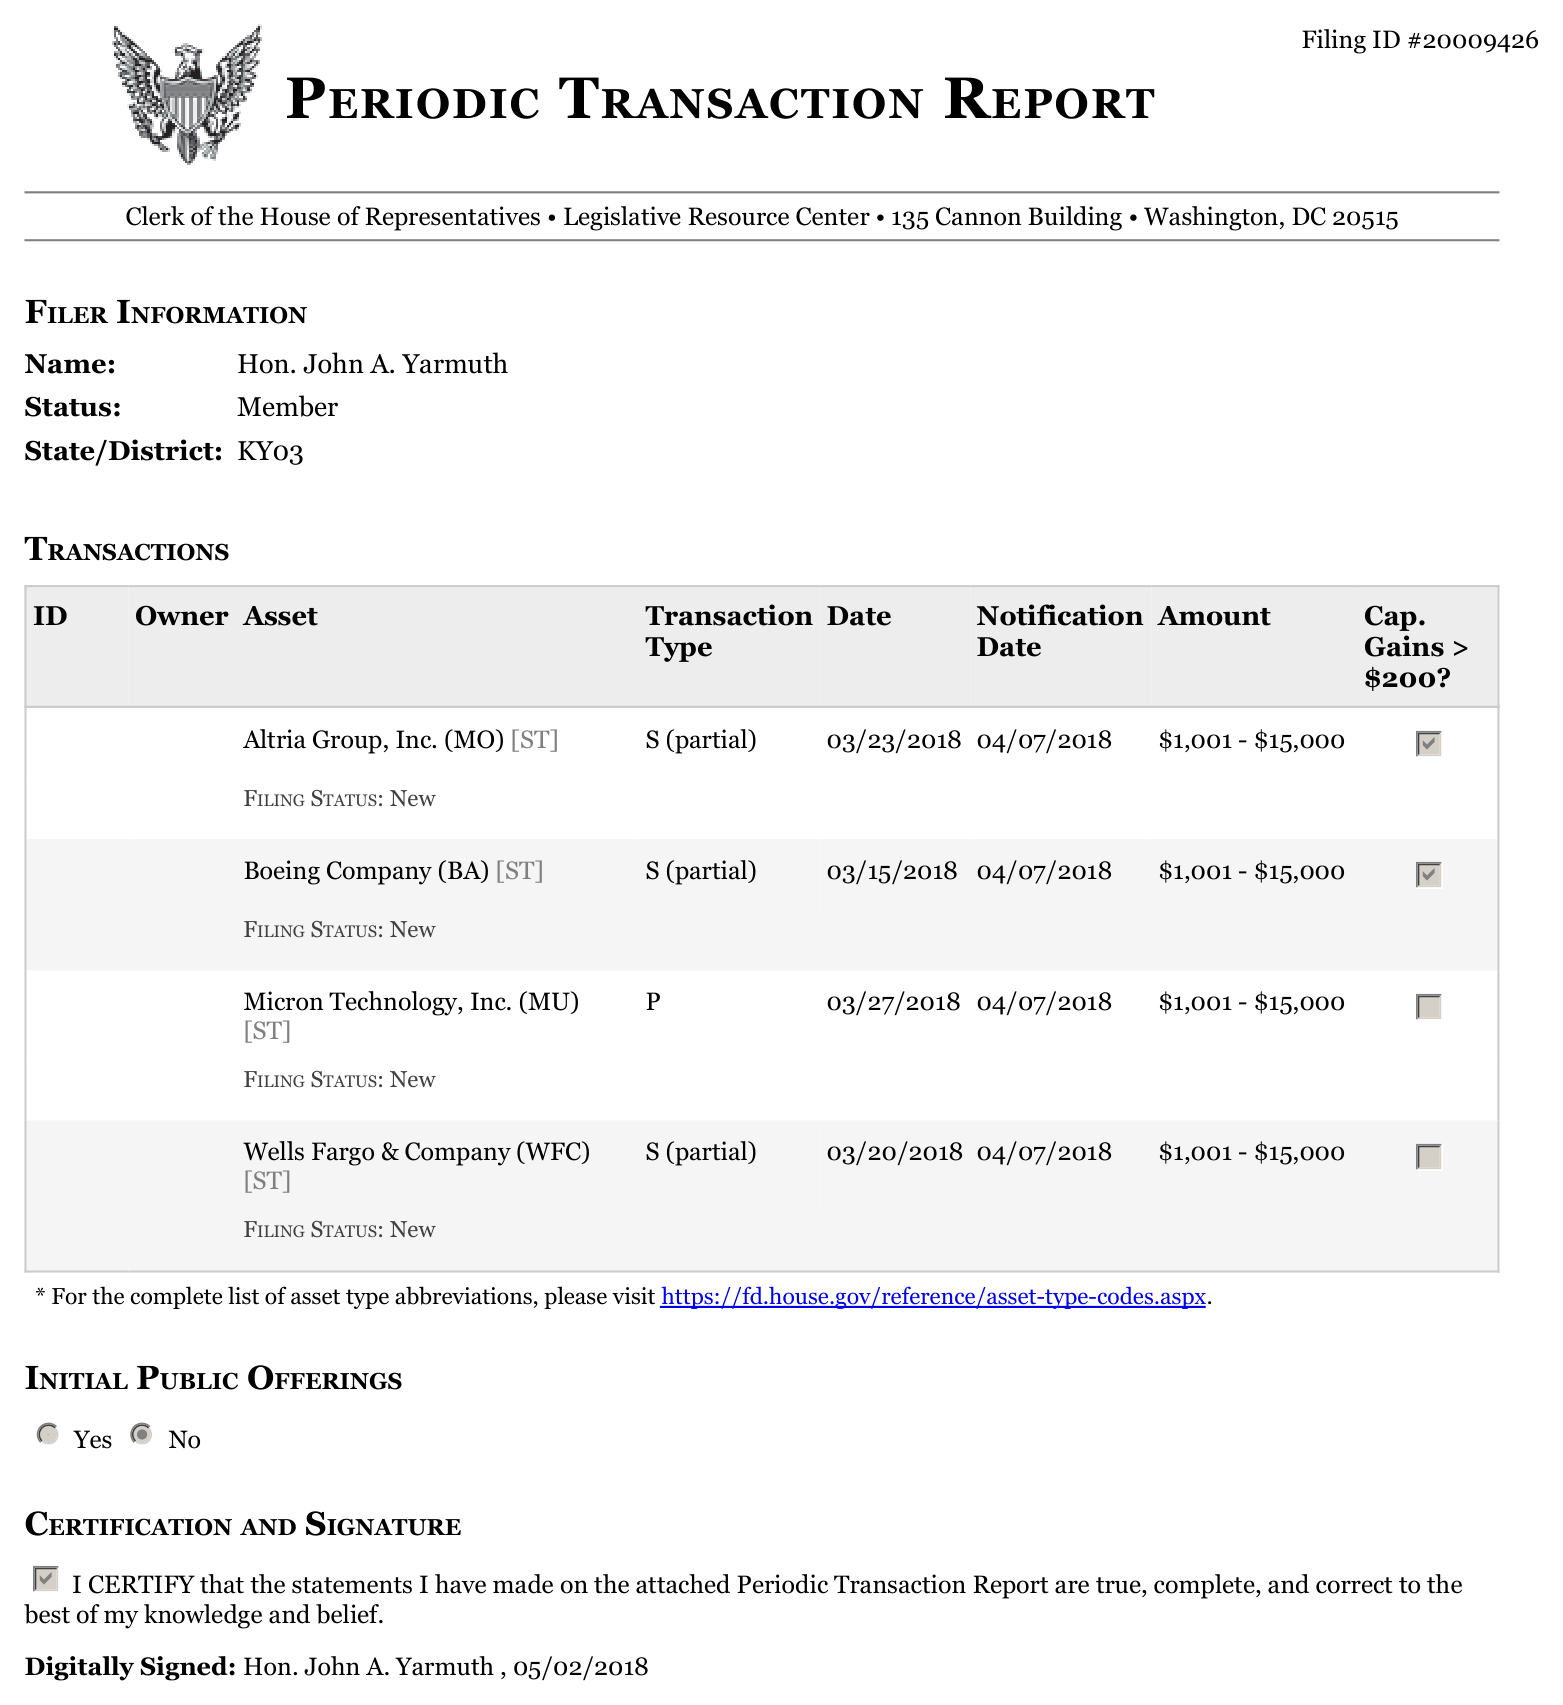
\includegraphics[height=42mm]{slides/fig_ptr_digital.png}}\\[1mm]
      {\footnotesize\textbf{LISIBLE} — identifiant en \co{1/2/3/4}\\
       {\scriptsize du vrai texte : on le parse directement}}
    \end{column}
    \begin{column}{0.48\textwidth}\centering
      \fcolorbox{black!25}{white}{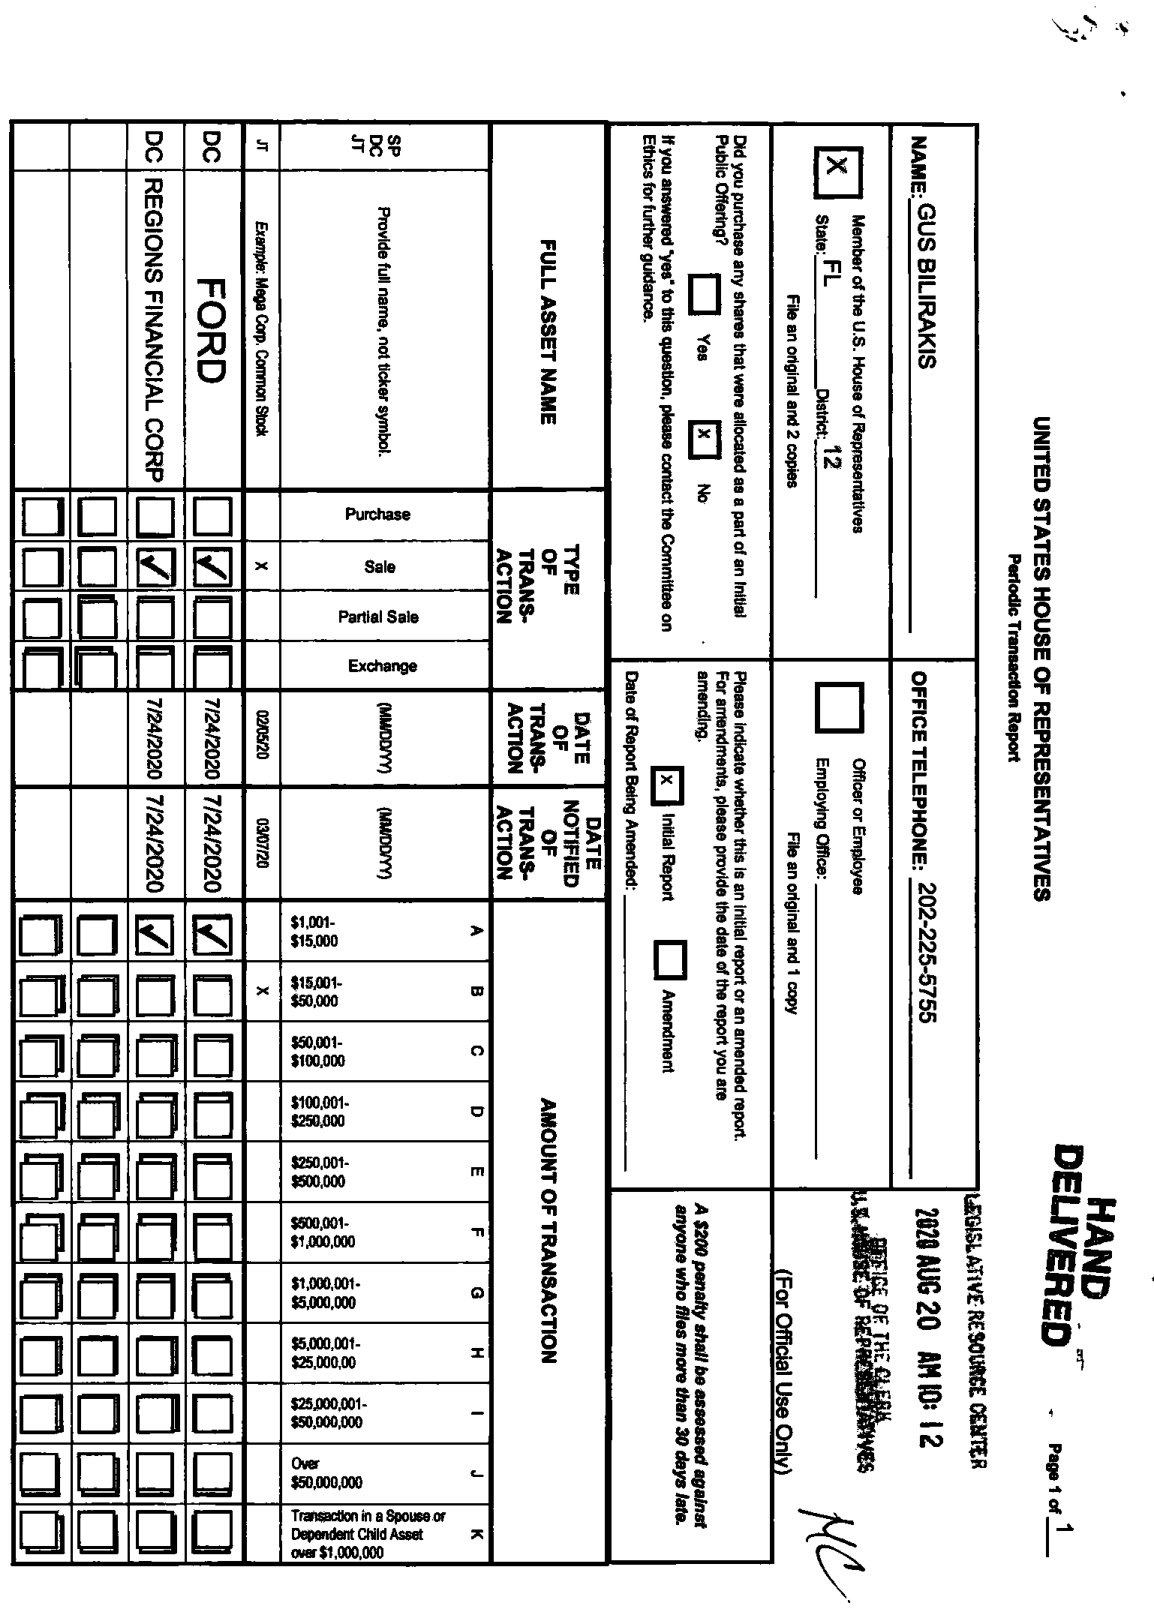
\includegraphics[height=42mm]{slides/scan_full_couche.png}}\\[1mm]
      {\footnotesize\textbf{SCANNÉ} — identifiant en \co{7/8/9}\\
       {\scriptsize une image (parfois manuscrite) : il faut de l'OCR}}
    \end{column}
  \end{columns}
\end{frame}

% ── S6 · Prouvé + le ledger ── (tables 02/03)
\begin{frame}{Vérifié sur les 26\,088 PDF — zéro désaccord}
  \centering
  {\footnotesize on ne croit pas l'identifiant sur parole : pour chaque PDF, on
   regarde s'il contient réellement du texte}\\[3mm]
  {\normalsize\setlength{\tabcolsep}{12pt}\renewcommand{\arraystretch}{1.3}
  \begin{tabular}{l cc}
    \toprule
    & annoncé lisible & annoncé scanné \\
    \midrule
    contient du texte & \textcolor{okgreen}{\textbf{20\,821}} & \textcolor{alertred}{\textbf{0}} \\
    image seulement & \textcolor{alertred}{\textbf{0}} & \textcolor{okgreen}{\textbf{5\,267}} \\
    \bottomrule
  \end{tabular}}\\[4mm]
  \badge{okgreen}{le tri lisible/scanné n'est pas une hypothèse : c'est une mesure}\\[2mm]
  {\scriptsize\color{black!60} et chaque dépôt reçoit UN statut dans un registre
   (le « ledger ») dont la somme retombe exactement sur 35\,377 — rien ne se perd}
\end{frame}

\section{Étape 3 · Identifier — du nom imprimé à l'élu}
% ── S7 · Identité ── (MANIFEST identité)
\begin{frame}{Relier tous les documents d'un même élu}
  \centering
  {\footnotesize l'index ne donne qu'un \textbf{nom imprimé} (« PELOSI, Nancy —
   CA11 ») ; pour croiser transactions ↔ rapports annuels ↔ entrée ↔ sortie,
   chaque dépôt est rattaché à l'\textbf{identifiant officiel} de l'élu au
   Congrès}\\[4mm]
  \badge{okgreen}{transactions : 99,9 \% rattachées}\;
  \badge{okgreen}{annuels : 98,9 \%}\;
  \badge{okgreen}{entrées : 99,2 \%}\;
  \badge{okgreen}{sorties : 99,2 \%}\\[2mm]
  \badge{okgreen}{zéro cas ambigu sur les transactions — garde anti-homonyme par l'État}\\[4mm]
  {\scriptsize\color{black!60} 1\,443 déclarants
   rattachés · les candidats jamais élus n'ont pas d'identifiant au Congrès
   ($\approx$ 90 \% des rapports de candidature) — c'est attendu, pas un défaut}
\end{frame}

\section{Étape 4 · Le cycle de vie — qui entre, qui sort, qui reste}
% ── S8 · La frise C→H→P→O/A→T ──
\begin{frame}{Les six dépôts d'une carrière}
  \centering
  \resizebox{0.97\textwidth}{!}{%
  \begin{tikzpicture}[node distance=7mm]
    \node[step=dataC, text width=2.5cm, minimum height=1.7cm, font=\footnotesize] (c)
      {\textbf{C} · candidat\\{\scriptsize photo du patrimoine\\avant l'élection}};
    \node[step=okgreen, text width=2.5cm, minimum height=1.7cm, font=\footnotesize, right=of c] (h)
      {\textbf{H} · entrée\\{\scriptsize photo du patrimoine\\en prenant le poste}};
    \node[step=helec, text width=2.9cm, minimum height=1.7cm, font=\footnotesize, right=of h] (p)
      {\textbf{P} · transactions\\{\scriptsize chaque achat/vente,\\déclaré sous 45 jours}};
    \node[step=dataC, text width=2.7cm, minimum height=1.7cm, font=\footnotesize, right=of p] (o)
      {\textbf{O} · annuel\\{\scriptsize bilan de l'année\\(corrigé par \textbf{A})}};
    \node[step=okgreen, text width=2.5cm, minimum height=1.7cm, font=\footnotesize, right=of o] (t)
      {\textbf{T} · sortie\\{\scriptsize photo du patrimoine\\en quittant le poste}};
    \draw[arr] (c) -- (h); \draw[arr] (h) -- (p); \draw[arr] (p) -- (o); \draw[arr] (o) -- (t);
  \end{tikzpicture}}\\[4mm]
  {\footnotesize\badge{helec}{les photos (C, H, O, T) disent CE QU'IL POSSÈDE ·
   les P disent CE QU'IL FAIT}}\\[2mm]
  {\scriptsize\color{black!60} C et H sont des photos pures : le formulaire
   n'y demande pas de transactions}
\end{frame}

% ── S9 · Entrées / sorties ── (source : §15.2 du notebook, vérifié adversarialement)
\begin{frame}{Qui dépose quoi — la couverture réelle}
  \centering
  {\footnotesize\setlength{\tabcolsep}{10pt}\renewcommand{\arraystretch}{1.25}
  \begin{tabular}{l l}
    \toprule
    \textbf{470 entrées} au Congrès & 82 \% ont déposé un H \\
    (depuis 2014) & 16 \% un C à la place (la loi les en dispense) \\
    & 2 \% ni l'un ni l'autre → \textbf{98 \% couverts} \\
    \midrule
    \textbf{463 sorties} définitives & 81 \% ont déposé un T \\
    & 86 sans T : partis au Sénat ou à l'exécutif \\
    & (dispensés), décès, départs trop récents \\
    \bottomrule
  \end{tabular}}\\[3.5mm]
  {\footnotesize presque chaque entrée a sa photo — mais une entrée sur cinq
   qui sort ne laisse pas de photo de sortie}
\end{frame}

% ── S10 · Le quadrant ── (table 14, colonne quadrant)
\begin{frame}{Les 900 membres de la fenêtre — qui peut-on tester de bout en bout ?}
  \centering
  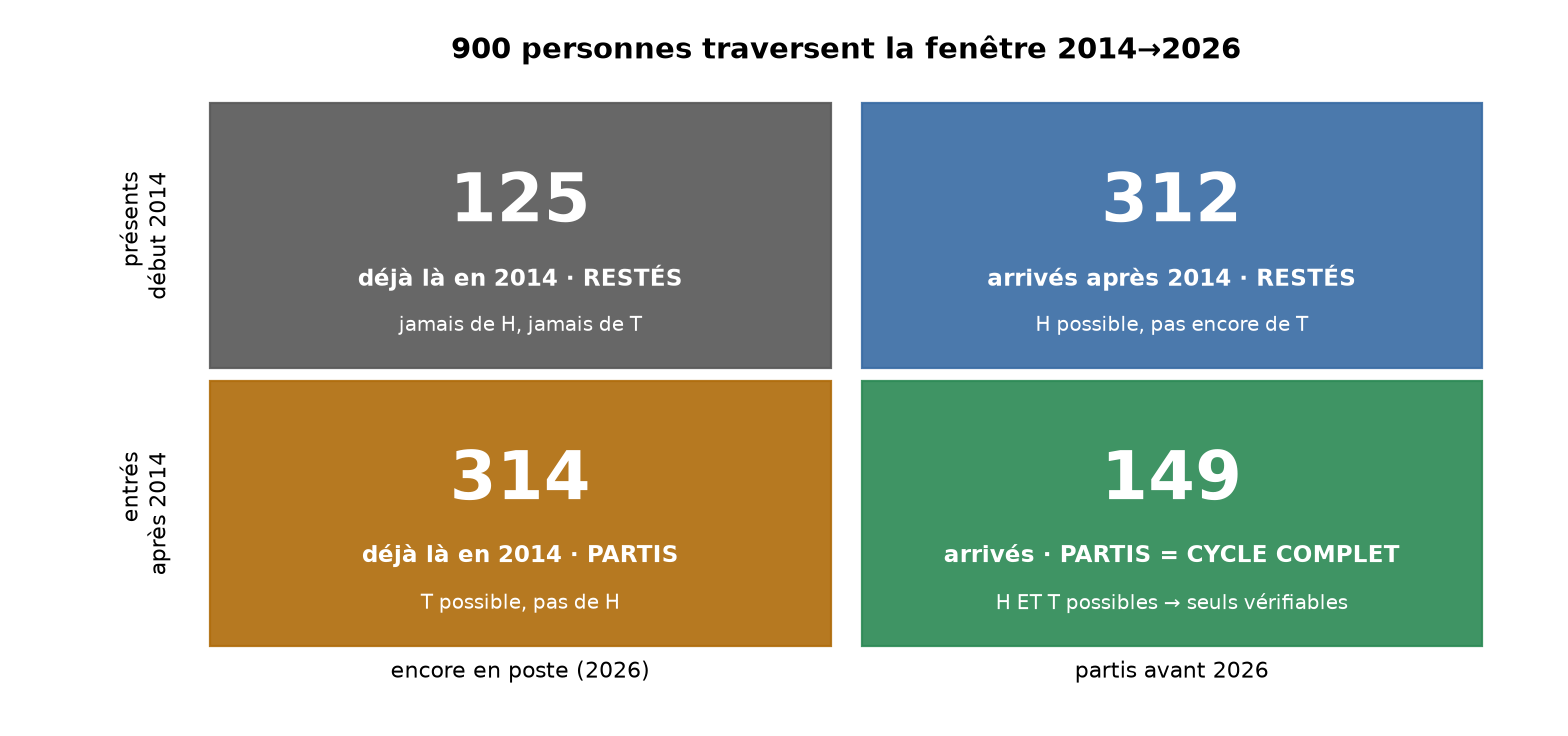
\includegraphics[width=0.70\textwidth]{fig_house_quadrant.png}\\[1.5mm]
  {\footnotesize les 439 déjà en poste en 2014 n'ont pas de photo d'entrée ·
   les 437 encore en poste n'ont pas de photo de sortie →
   \textbf{seuls les 149 entrés PUIS sortis} peuvent être vérifiés
   de bout en bout}
\end{frame}

\section{Étape 5 · Extraire — le patrimoine et les transactions}
% ── S11 · Sections A→J ──
\begin{frame}{Dans chaque document, dix sections — on n'en exploite que deux}
  \centering
  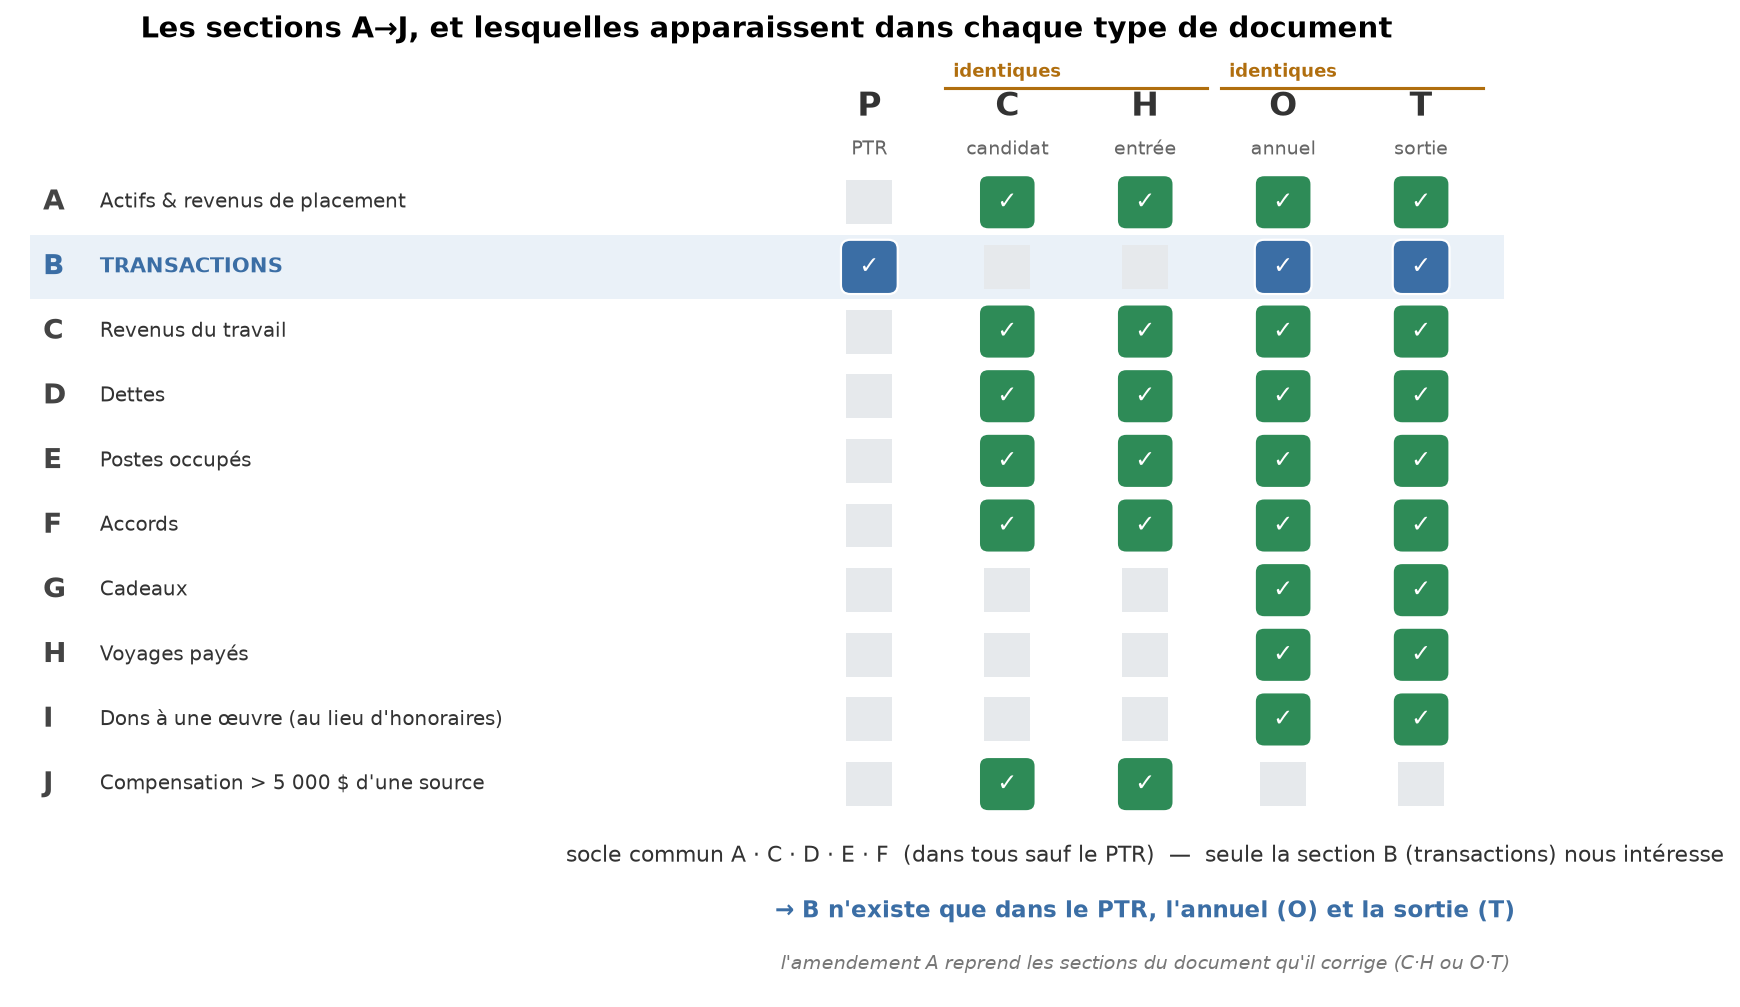
\includegraphics[width=0.80\textwidth]{slides/fig_sections_matrix.png}\\[2mm]
  {\footnotesize \badge{dataC}{Schedule A = le PATRIMOINE (les photos)}\;
   \badge{helec}{Schedule B = les TRANSACTIONS}}\\[1.5mm]
  {\scriptsize\color{black!60} le reste (salaires, dettes, cadeaux, voyages…)
   est hors sujet pour un signal de trading}
\end{frame}

% ── S12 · Les 4 canaux ── (tables 04/05/07/08/09)
\begin{frame}{Quatre canaux d'extraction — électronique d'abord, OCR pour le reste}
  \centering
  \tuile{dataC}{198\,615}{photos de patrimoine\\électroniques}\hfill
  \tuile{helec}{56\,002}{transactions P\\électroniques}\hfill
  \tuile{helec}{110\,147}{transactions des\\annuels (électroniques)}\hfill
  \tuile{hocr}{449\,350}{lignes lues par OCR\\(tout le scanné)}\\[4mm]
  {\footnotesize \badge{okgreen}{rien de lisible ne part inutilement en OCR —
   et zéro document scanné n'a été laissé de côté}}\\[2mm]
  {\scriptsize\color{black!60} OCR = 105\,074 transactions P +
   188\,970 photos + 155\,306 transactions d'annuels,
   lues par vision automatique sur les documents papier}
\end{frame}

% ── S13 · Totaux ── (MANIFEST + tables ; 28 j = médiane vérifiée)
\begin{frame}{Ce que l'extraction livre}
  \centering
  \tuile{okgreen}{161\,076}{transactions datées\\= LE SIGNAL}\hfill
  \tuile{helec}{28 j}{délai médian\\trade → publication}\hfill
  \tuile{dataC}{387\,585}{photos de patrimoine\\(toutes sources)}\\[4mm]
  {\footnotesize le signal, c'est les P : les seules transactions connues assez
   vite pour être tradées. Tout le reste — photos et transactions des annuels —
   sert à \textbf{reconstruire et vérifier} les portefeuilles.}
\end{frame}

\section{Étape 6 · Le portefeuille d'entrée}
% ── S14 · La photo de départ ── (table 15)
\begin{frame}{La photo de départ de chaque membre}
  \centering
  \tuile{okgreen}{252}{membres ancrés\\par leur H}\hfill
  \tuile{dataC}{32}{ancrés par leur C\\(dispensés de H)}\hfill
  \tuile{helec}{284}{= portefeuilles\\d'entrée datés}\hfill
  \tuile{grisC}{616}{sans photo d'entrée\\(déjà en poste en 2014…)}\\[4mm]
  {\footnotesize un C n'est accepté comme photo de départ que sous
   \textbf{trois garde-fous} : électronique · au moins une action cotée ·
   déposé moins d'un an avant la prise de poste (le C de campagne d'un élu
   déjà en place ne compte pas)}\\[2mm]
  {\scriptsize\color{black!60} sans H ni C, la reconstruction s'ancre sur le
   premier rapport annuel — plus tardif, donc série partielle}
\end{frame}

\section{Étape 7 · Les flux, dédupliqués}
% ── S15 · Dédup à l'assemblage ── (source : §10 du notebook — 189 117 → 166 149)
\begin{frame}{Les transactions ne vivent pas que dans les P}
  \centering
  {\footnotesize les annuels, les amendements et les rapports de sortie déclarent
   AUSSI des transactions — souvent les mêmes, re-déclarées}\\[4mm]
  \resizebox{0.9\textwidth}{!}{%
  \begin{tikzpicture}[node distance=9mm]
    \node[step=helec, text width=3.2cm, minimum height=1.5cm, font=\footnotesize] (a)
      {\textbf{189\,117} lignes\\{\scriptsize toutes sources électroniques}};
    \node[step=dataC, text width=3.4cm, minimum height=1.5cm, font=\footnotesize, right=of a] (b)
      {\textbf{−\,22\,968} doublons\\{\scriptsize le même trade re-déclaré\\(annuel, amendement…)}};
    \node[step=okgreen, text width=3.2cm, minimum height=1.5cm, font=\footnotesize, right=of b] (c)
      {\textbf{166\,149} uniques\\{\scriptsize chaque trade compté\\UNE fois}};
    \draw[arr] (a) -- (b); \draw[arr] (b) -- (c);
  \end{tikzpicture}}\\[4mm]
  {\footnotesize la déduplication se fait ICI, à l'assemblage — là où toutes les
   sources se rencontrent ; on garde la première divulgation publique}
\end{frame}

% ── S16 · Le gain net des annuels ── (table 16)
\begin{frame}{Ce que les annuels apportent en plus — et pourquoi ce n'est pas du signal}
  \centering
  \tuile{okgreen}{26\,115}{trades jamais vus\\dans un P}\hfill
  \tuile{dataC}{22\,216}{via les annuels}\hfill
  \tuile{dataC}{3\,899}{via sorties et\\amendements}\hfill
  \tuile{grisC}{374 j}{délai médian\\trade → publication}\\[4mm]
  {\footnotesize ces trades comblent des trous du portefeuille (des élus oublient
   leur déclaration P mais les inscrivent à l'annuel) — mais on les découvre
   \textbf{un an trop tard} : ils nourrissent le patrimoine, jamais le signal}
\end{frame}

\section{Étape 8 · Vérifier — entrée + achats ⊇ sortie}
% ── S17 · Le test ──
\begin{frame}{Le test de cohérence — la chronologie d'un mandat doit se recouper}
  \centering
  {\footnotesize chaque position détenue à la SORTIE doit s'expliquer :
   soit elle était là à l'ENTRÉE, soit elle a été ACHETÉE entre les deux}\\[4mm]
  \resizebox{0.93\textwidth}{!}{%
  \begin{tikzpicture}[node distance=8mm]
    \node[step=okgreen, text width=3.0cm, minimum height=1.6cm, font=\footnotesize] (h)
      {\textbf{photo d'ENTRÉE}\\{\scriptsize ce qu'il possède\\en arrivant}};
    \node[step=helec, text width=3.2cm, minimum height=1.6cm, font=\footnotesize, right=of h] (p)
      {\textbf{+ les ACHATS}\\{\scriptsize toutes les transactions\\du mandat}};
    \node[step=dataC, text width=3.2cm, minimum height=1.6cm, font=\footnotesize, right=of p] (t)
      {\textbf{doit couvrir la SORTIE}\\{\scriptsize chaque position,\\une par une}};
    \draw[arr] (h) -- (p); \draw[arr] (p) -- (t);
  \end{tikzpicture}}\\[4mm]
  {\scriptsize\color{black!60} quatre déclarations INDÉPENDANTES du même
   portefeuille (entrée, transactions, annuels, sortie) : si la collecte était
   trouée, ça se verrait ici}
\end{frame}

% ── S18 · La cohorte testable ── (quadrant + photos + tickers)
\begin{frame}{Sur qui peut-on faire ce test ?}
  \centering
  \resizebox{0.9\textwidth}{!}{%
  \begin{tikzpicture}[node distance=9mm]
    \node[step=grisC, text width=3.2cm, minimum height=1.6cm, font=\footnotesize] (a)
      {\textbf{149} cycles complets\\{\scriptsize entrés PUIS sortis\\dans la fenêtre}};
    \node[step=dataC, text width=3.2cm, minimum height=1.6cm, font=\footnotesize, right=of a] (b)
      {\textbf{106} avec les\\deux photos déposées\\{\scriptsize entrée ET sortie}};
    \node[step=okgreen, text width=3.4cm, minimum height=1.6cm, font=\footnotesize, right=of b] (c)
      {\textbf{56} testables\\{\scriptsize des actions cotées\\des deux côtés}};
    \draw[arr] (a) -- (b); \draw[arr] (b) -- (c);
  \end{tikzpicture}}\\[4mm]
  {\footnotesize la moitié des membres à double photo ne détient \textbf{aucune
   action cotée} (fonds, immobilier, comptes gérés) — on ne peut pas suivre
   ce qui n'a pas de cours de bourse : c'est la nature du patrimoine,
   pas un défaut de collecte}
\end{frame}

% ── S19 · Le résultat ── (MANIFEST : 78,7 / 87,8 / 3,3 ; élargie 87,1)
\begin{frame}{Le résultat — les portefeuilles se recoupent}
  \centering
  \tuile{helec}{78,7 \%}{expliqué par les\\transactions P seules}\hfill
  \tuile{okgreen}{87,8 \%}{avec TOUTES les\\déclarations}\hfill
  \tuile{alertred}{3,3 \%}{vraiment\\inexpliqué}\\[4mm]
  {\footnotesize l'écart entre les deux premiers chiffres, c'est surtout du
   \textbf{non-dépôt documenté} : l'élu a déclaré l'achat dans son annuel,
   jamais dans un P — quelques habitués concentrent l'essentiel}\\[2.5mm]
  {\scriptsize\color{black!60} deux limites assumées : les montants sont des
   \textbf{fourchettes sans quantités} (on vérifie la présence d'un titre, pas un
   solde comptable) · les blind trusts ne créent pas de faux trous — le
   portefeuille y devient invisible, il ne fuit pas ·
   la cohorte élargie au papier confirme (87,1 \%)}
\end{frame}

\section{Étape 9 · Reconstruire — le portefeuille daté de chaque membre}
% ── S20 · Le moteur ── (tables 12/13)
\begin{frame}{Le moteur — photo, flux, recalage}
  \centering
  \resizebox{0.93\textwidth}{!}{%
  \begin{tikzpicture}[node distance=8mm]
    \node[step=okgreen, text width=3.0cm, minimum height=1.6cm, font=\footnotesize] (a)
      {\textbf{photo d'ancrage}\\{\scriptsize la photo d'entrée,\\ou la 1re disponible}};
    \node[step=helec, text width=3.2cm, minimum height=1.6cm, font=\footnotesize, right=of a] (b)
      {\textbf{+ flux datés}\\{\scriptsize achats et ventes,\\appliqués jour par jour}};
    \node[step=dataC, text width=3.4cm, minimum height=1.6cm, font=\footnotesize, right=of b] (c)
      {\textbf{recalage}\\{\scriptsize à chaque nouvelle photo,\\le document fait foi}};
    \draw[arr] (a) -- (b); \draw[arr] (b) -- (c);
    \draw[arr, bend right=25] (c.south) to (b.south);
  \end{tikzpicture}}\\[4mm]
  \tuile{helec}{825}{membres avec un\\portefeuille daté}\hfill
  \tuile{dataC}{6\,049}{photos de patrimoine\\dans leurs séries}\hfill
  \tuile{okgreen}{66,7 \%}{des positions confirmées\\d'une photo à l'autre}\\[2mm]
  {\scriptsize\color{black!60} en positions et en fourchettes de valeur —
   jamais en quantités : la loi ne les publie pas}
\end{frame}

% ── S21 · Le registre ── (table 14)
\begin{frame}{Un statut explicite pour chacun des 900 membres}
  \centering
  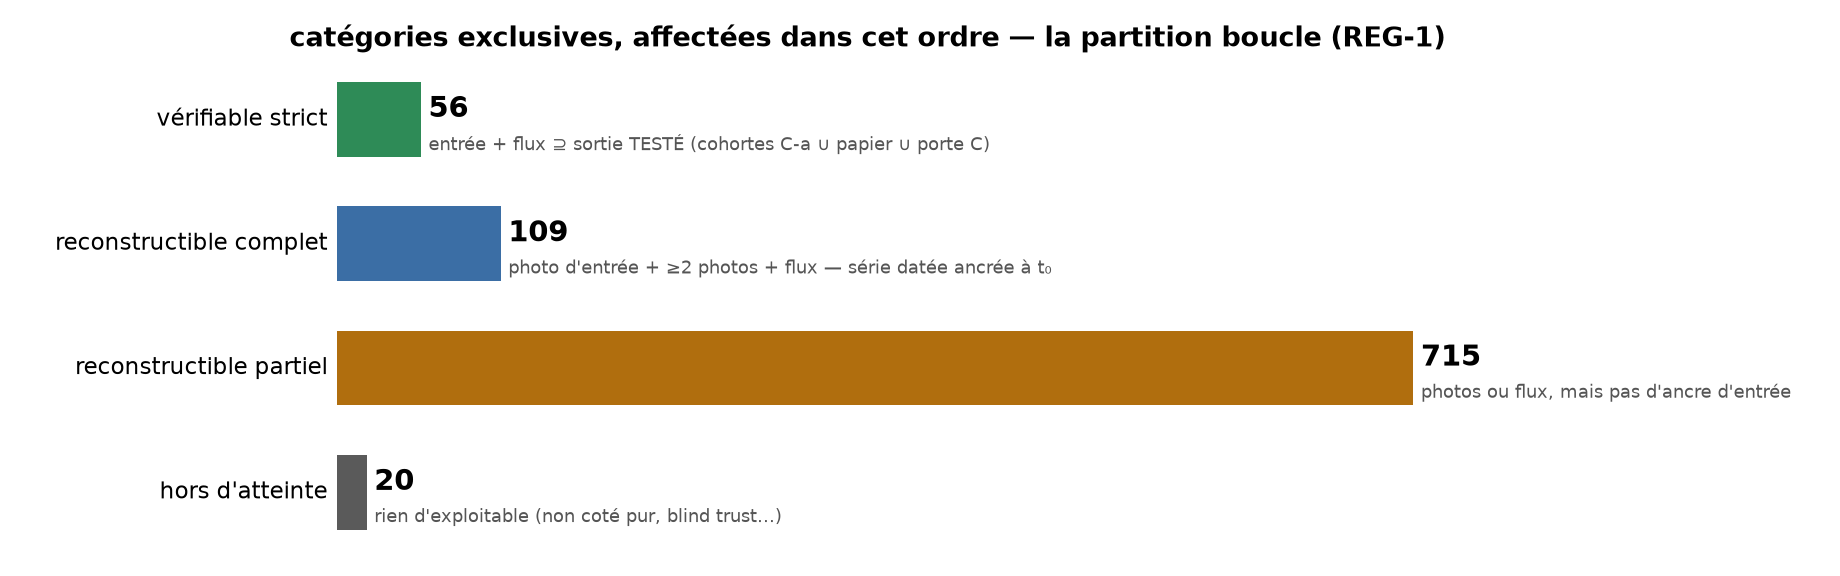
\includegraphics[width=0.9\textwidth]{fig_house_registre.png}\\[2mm]
  {\footnotesize « le portefeuille de chaque membre » se dit honnêtement :
   qui est \textbf{vérifié}, qui est \textbf{reconstruit avec son point de
   départ}, qui est \textbf{partiel}, qui est \textbf{hors d'atteinte} —
   et pourquoi, membre par membre}
\end{frame}

% ── S22 · Les deux compteurs ── (MANIFEST + table 18)
\begin{frame}{Les deux compteurs — reconstruire n'est pas vérifier}
  \centering
  \tuile{helec}{825}{portefeuilles\\RECONSTRUITS}\hfill
  \tuile{okgreen}{56}{portefeuilles VÉRIFIÉS\\de bout en bout}\\[4mm]
  {\footnotesize ces deux nombres ne s'additionnent ni ne se comparent : pour
   $\approx$ 9 membres sur 10, on reconstruit la série sans pouvoir la vérifier
   entrée → sortie (pas de cycle complet, ou pas d'actions cotées)}\\[2.5mm]
  {\scriptsize\color{black!60} et ce qui ne colle pas entre deux photos est
   \textbf{publié et décomposé}, pas caché — l'essentiel vient des libellés
   d'actifs qui changent d'écriture d'une année à l'autre (la suite naturelle :
   un appariement tolérant aux variations de nom)}
\end{frame}

\section{Étape 10 · Rien d'oublié}
% ── S23 · La comptabilité ── (table 10)
\begin{frame}{Chaque dépôt a un traitement — la somme boucle}
  \centering
  
\includegraphics[width=0.86\textwidth]{fig_house_compta.png}\\[2mm]
  {\footnotesize \badge{okgreen}{la somme retombe exactement sur 35\,377}\;
   \badge{okgreen}{zéro document scanné laissé de côté}\;
   \badgel{grisC!25}{\textcolor{grisC}{\textbf{10 exclus : des PDF morts côté
   site, tracés un par un}}}}
\end{frame}

% ── S24 · Les contrôles ── (MANIFEST : 75 validations, 0 rouge)
\begin{frame}{Tout est contrôlé, tout est re-jouable}
  \centering
  \tuile{okgreen}{75}{contrôles automatiques\\dans le notebook}\hfill
  \tuile{helec}{0}{contrôle\\en échec}\hfill
  \tuile{dataC}{18}{tables versionnées\\(chaque chiffre traçable)}\\[4mm]
  {\footnotesize chaque affirmation de ce deck sort d'un contrôle du notebook :
   un chiffre faux ferait échouer l'exécution. Relancer le notebook rejoue
   TOUT — téléchargements, extraction, vérifications — à l'identique.}
\end{frame}

\section{Verdict}
% ── S25 · Verdict ──
\begin{frame}{Ce que ce travail prouve — et la suite}
  \centering
  {\footnotesize
  \badge{helec}{1. la source est exhaustive et ARCHIVÉE — c'est le site qui efface, pas nous}\\[2mm]
  \badge{helec}{2. le tri lisible/scanné est MESURÉ — et tout le scanné a été lu}\\[2mm]
  \badge{helec}{3. les portefeuilles SE RECOUPENT — 87,8 \% expliqué,
   3,3 \% d'inexpliqué résiduel}}\\[5mm]
  \tuile{okgreen}{161\,076}{transactions datées\\= le signal, complet}\hfill
  \tuile{dataC}{825}{portefeuilles\\reconstruits et datés}\hfill
  \tuile{helec}{56}{vérifiés\\de bout en bout}\\[4mm]
  {\scriptsize\color{black!60} la suite : le Sénat sur le même plan ·
   l'appariement tolérant des noms d'actifs · brancher le portefeuille d'entrée
   dans le moteur de stratégie}
\end{frame}

\end{document}
